\immediate\write18{tex tqft.dtx}
\documentclass{ltxdoc}
\usepackage[T1]{fontenc}
\usepackage{lmodern}
\usepackage{morefloats}
\usepackage[svgnames]{xcolor}
\usepackage{tikz}
\usepackage{tqft}
\usepackage[numbered]{hypdoc}
\definecolor{lstbgcolor}{rgb}{0.9,0.9,0.9} 
 
\usepackage{listings}
\lstloadlanguages{[LaTeX]TeX}
\lstset{breakatwhitespace=true,breaklines=true,language=TeX}
 
\usepackage{fancyvrb}

\newenvironment{example}
  {\VerbatimEnvironment
   \begin{VerbatimOut}{example.out}}
  {\end{VerbatimOut}
   \begin{center}
   \setlength{\parindent}{0pt}
   \fbox{\begin{minipage}{.9\linewidth}
     \lstset{breakatwhitespace=true,breaklines=true,language=TeX,basicstyle=\small}
     \lstinputlisting[]{example.out}
   \end{minipage}}

   \fbox{\begin{minipage}{.9\linewidth}
     \centering
     \input{example.out}
   \end{minipage}}
\end{center}
}

\providecommand*{\url}{\texttt}
\GetFileInfo{tqft.sty}

\title{The \textsf{tqft} Package: Documentation}
\author{Andrew Stacey \\ \url{stacey@math.ntnu.no}}
\date{\fileversion~from \filedate}

\begin{document}

\maketitle

\begin{center}

\begin{tikzpicture}[scale=.5,every tqft/.style={fill=DarkMagenta,draw,ultra thick},every node/.style={tqft cobordism,transform shape}]
  \node[
    tqft,
    incoming boundary components=0,
    outgoing boundary components=3,
  ] (a) {};
  \node[
    tqft cylinder,
    anchor=incoming boundary 1,
  ] at (a.outgoing boundary 2) (b) {};
  \node[
    tqft,
    incoming boundary components=0,
    outgoing boundary components=2,
    anchor=outgoing boundary 1,
  ] at (a outgoing 3.next) (c) {};
  \node[
    tqft,
    incoming boundary components=3,
    outgoing boundary components=1,
    offset=2.5,
    anchor=incoming boundary 1,
    boundary separation=1cm,
    cobordism height=2.5cm,
  ] at (c.outgoing boundary 1) (d) {};
  \node[
    tqft,
    flow=east,
    incoming boundary components=0,
    outgoing boundary components=3,
  ] at (c outgoing 2.next) (e) {};
  \node[
    tqft cylinder,
    flow=east,
    anchor=incoming boundary 1,
  ] at (e.outgoing boundary 1) (f) {};
  \node[
    tqft cylinder,
    flow=east,
    anchor=incoming boundary 1,
  ] at (e.outgoing boundary 2) (g) {};
  \node[
    tqft,
    incoming boundary components=0,
    outgoing boundary components=3,
    anchor=outgoing boundary 1,
  ] at (g outgoing 1.below) (h) {};
  \node[
    tqft cylinder,
    anchor=incoming boundary 1,
  ] at (h.outgoing boundary 2) (i) {};
\end{tikzpicture}
\end{center}

\section{Introduction}
This package defines some TikZ/PGF node shapes that can be used to construct the diagrams common in Topological Quantum Field Theory (TQFT).
An example follows:

\begin{example}
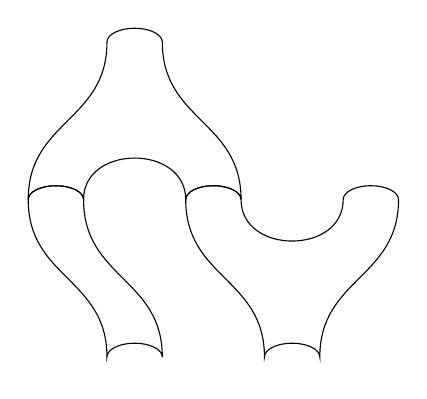
\begin{tikzpicture}
\node[draw,tqft/pair of pants] (a) {};
\node[draw,tqft/cylinder to next,anchor=incoming boundary 1] (c) at (a.outgoing boundary 1) {};
\node[draw,tqft/reverse pair of pants, anchor=incoming boundary 1] at (a.outgoing boundary 2) (b) {};
\end{tikzpicture}
\end{example}

Before giving any details, a word is in order about the keys involved in this package.
There are many options and keys that can be set via the \Verb+\pgfkeys+ system (which is used for setting options in Ti\emph{k}Z).
Such keys live in a ``directory'' but often that can be omitted.
For example, in the Ti\emph{k}Z command \Verb+\draw[red] (0,0) -- (1,0);+ the key \Verb+red+ is actually in the ``directory'' \Verb+/tikz+ but it is not necessary to specify that as it is assumed.
Defining a ``directory'' helps separate keys and ensure that there is no conflict.
The keys in this package are (mostly) defined in the directory \Verb+/pgf/tqft+ but the very first call to a \Verb+tqft+ key will (in general) set the ``current directory'' to \Verb+/pgf/tqft+ and so all subsequent keys do not need prefixing.
Moreover, any unknown keys are passed on to the \Verb+/tikz+ directory so there is (or should be!) no harm in mixing \Verb+tqft+ specific keys with ordinary Ti\emph{k}Z keys.
Some examples take advantage of this switch so when copying and modifying examples from this document, it is important to remember that the first \Verb+tqft+ specific key needs an explicit \Verb+tqft/+ prefix.
More detailed information is in the section on styling.

\section{The Shapes}

There are only two shapes, \Verb+tqft cobordism+ and \Verb+tqft boundary circle+.
The first, which is the main shape, is a cobordism between a number of incoming circles and a number of outgoing circles, where the numbers of boundary components can be specified as options to the shape.
The second is just the boundary circle.
It is used as a sub-node of the first to add extra anchors, but can be used by itself.
There are certain common shapes that are predefined as aliases to the main shape with specified boundaries.
The list of predefined shapes follows.
The names are all in the \Verb+tqft+ family, but an alias is made so that \Verb+tqft nodeshape+ will work without any further qualification.

\begin{enumerate}
\item \Verb+pair of pants+

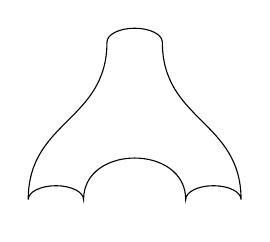
\begin{tikzpicture}
\node[draw,tqft/pair of pants] (a) {};
\end{tikzpicture}

\item \Verb+reverse pair of pants+

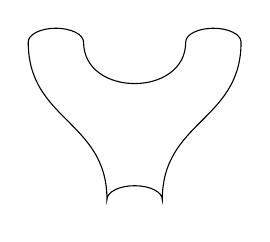
\begin{tikzpicture}
\node[draw,tqft/reverse pair of pants] (a) {};
\end{tikzpicture}

\item \Verb+cylinder to prior+

This is a cylinder that has been skewed to one side, thus following the same path as the \Verb+pair of pants+ cobordism but with only one outgoing boundary component.
The name \Verb+to prior+ is because it goes towards the lower-numbered component on the \Verb+pair of pants+. 

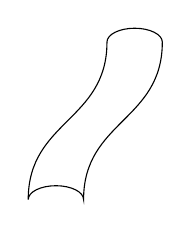
\begin{tikzpicture}
\node[draw,tqft/cylinder to prior] (a) {};
\end{tikzpicture}

\item \Verb+cylinder to next+

This is a cylinder that has been skewed to one side, thus following the same path as the \Verb+pair of pants+ cobordism but with only one outgoing boundary component.
The name \Verb+to next+ is because it goes towards the higher-numbered component on the \Verb+pair of pants+. 

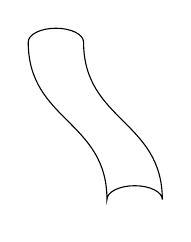
\begin{tikzpicture}
\node[draw,tqft/cylinder to next] (a) {};
\end{tikzpicture}

\item \Verb+cylinder+

This is a straight cylinder.

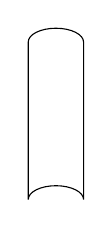
\begin{tikzpicture}
\node[draw,tqft/cylinder] (a) {};
\end{tikzpicture}

\item \Verb+cap+

This is a cap.

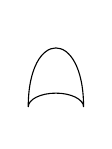
\begin{tikzpicture}
\node[draw,tqft/cap] (a) {};
\end{tikzpicture}

\item \Verb+cup+

This is a cup (an upside-down cap).

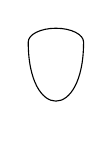
\begin{tikzpicture}
\node[draw,tqft/cup] (a) {};
\end{tikzpicture}

\end{enumerate}

The general shape is controlled by the following keys:

\begin{itemize}
\item \DescribeMacro{flow} A cobordism ``flows'' from its incoming to its outgoing boundaries.
This key controls the direction of that flow.
The shape is transformed so that the incoming-outgoing axis aligns with the argument.
However, the transformation may be more than just a rotation as the shape is set up so that the numbering of the boundary components is always left-to-right or top-to-bottom (as appropriate).
Currently, this key can take the values \Verb+north+, \Verb+south+ (default), \Verb+east+, and \Verb+west+.

\item \DescribeMacro{view from} To get a simulated 3D effect, the cobordism is drawn as if viewed from a slight angle.
The value of this key determines whether the cobordism is viewed from the direction of the incoming boundary components or the outgoing ones.
This key can take the values \Verb+incoming+ and \Verb+outgoing+.
The default is \Verb+outgoing+.
\item \DescribeMacro{cobordism height} This is the height of the cobordism (``height'' interpreted in its own internal coordinate system).
With no offset (q.v.), this would be the distance between the centres of the first incoming and first outgoing boundary components.

\item \DescribeMacro{boundary separation} This is the distance between the centres of the boundary components of the same type.

\item \DescribeMacro{circle width} This is the half-width of the boundary circles.

\item \DescribeMacro{circle depth} This is the half-depth of the boundary circles (``depth'' since, in the internal coordinate system, this corresponds to the \(z\)-axis out of the page).

\item \DescribeMacro{incoming boundary components} The number of incoming boundary components (can be zero).

\item \DescribeMacro{outgoing boundary components} The number of outgoing boundary components (can be zero).

\item \DescribeMacro{offset} This offsets the first outgoing boundary component horizontally relative to the first incoming boundary component.
It is a dimensionless number (not necessarily an integer) and is interpreted so that a value of \(1\) aligns the first outgoing boundary component with the second incoming boundary component.
\end{itemize}

\section{Styling}

There are various options for styling the diagrams.
To understand how they work, it is important to know the order in which a cobordism is drawn and how many pieces it decomposes into.
This is the following list, with the corresponding key:

\begin{enumerate}
\item The boundary circles are drawn.
\Verb+boundary style+
\item The lower edges of the boundary circles are redrawn.
\Verb+boundary lower style+
\item The cobordism itself is drawn.
\item The non-boundary edge of the cobordism is redrawn.
\Verb+cobordism style+
\item The upper edges of the boundary circles are redrawn.
\Verb+boundary upper style+
\end{enumerate}

The fact that there are so many is to allow different style to be applied to different pieces.
The duplication is to allow certain composite pieces to be \emph{filled}.
All of these items can be styled separately.
The style given to the node itself is passed on to the third item in that list, the cobordism itself.
The styles of the others are controlled by a series of keys, each of should be a list of styles to be applied to that component.
Not all options make sense, in particular only the first and third can be filled.
(That is, the \Verb+fill+ style is ignored on the other components.)
Here is a progressively built up cobordism.

\begin{example}
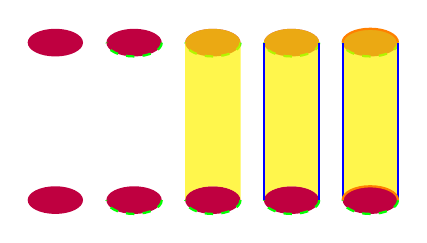
\begin{tikzpicture}
\begin{scope}[tqft/boundary style={fill=purple,fill opacity=1}]
\node[tqft/cylinder] at (1,0) {};
\begin{scope}[tqft/boundary lower style={draw,dashed,green,thick}]
\node[tqft/cylinder] at (2,0) {};
\begin{scope}
\node[tqft/cylinder,fill=yellow,fill opacity=.7] at (3,0) {};
\begin{scope}[tqft/cobordism style={draw,thick,blue}]
\node[tqft/cylinder,fill=yellow,fill opacity=.7] at (4,0) {};
\begin{scope}[tqft/boundary upper style={draw,thick,orange}]
\node[tqft/cylinder,fill=yellow,fill opacity=.7] at (5,0) {};
\end{scope}
\end{scope}
\end{scope}
\end{scope}
\end{scope}
\end{tikzpicture}
\end{example}

\section{Anchors}

As with all PGF node shapes, there are certain anchors defined by the \Verb+tqft+ shape.
These are the \Verb+center+ (and \Verb+centre+) anchors and the \Verb+incoming boundary n+, \Verb+outgoing boundary n+ anchors.
The positioning of the \Verb+center+ anchor is slightly unusual in that if there are no, say, incoming boundary components then the centre anchor is still at the same height above the outgoing boundary components as if there were incoming boundary components.
The reason for this is two-fold: computing the \emph{actual} centre of the shape in such circumstances would be tricky, and when aligning these shapes it is more useful to have the anchors consistent across shapes of varying boundary components.

There are also the directional anchors \Verb+north+, \Verb+south+, \Verb+east+, \Verb+west+, \Verb+north east+, \Verb+north west+, \Verb+south east+, \Verb+south west+.
The \Verb+east+ and \Verb+west+ anchors are placed at the midpoints of the sides.
The \Verb+north+ and \Verb+south+ anchors are placed in a vertical line with the \Verb+center+ anchor and vertically aligned with the centres of the corresponding boundary circles.
The other four directional anchors are placed at the corners of the cobordism (the placement of these anchors in the case that there are no boundary circles in the corresponding direction may change in future versions).

The \Verb+incoming boundary n+ and \Verb+outgoing boundary n+ are placed at the centres of the corresponding boundary components, with the numbering starting at the left or the top as appropriate to the flow of the cobordism.
A hack borrowed from the \Verb+regular polygon+ shape ensures that there are always enough anchors for the boundary components.

There are also anchors placed at the midpoint of the cobordism edge between the boundary circles.
The names of these are \Verb+after incoming boundary n+ and \Verb+after outgoing boundary n+.

The above anchors can all be ``floated'' off the cobordism using the keys \Verb+outer sep+, \Verb+outer xsep+, and \Verb+outer ysep+.
The last two are the ones actually used, the first is a shortcut for setting both simultaneously.

There are also ``sub-nodes''.
Provding the main node is named, each boundary circle is covered by a \Verb+tqft boundary circle+ node.
This means that the anchors of the \Verb+tqft boundary circle+ can be used.
These cannot be used for placing the main shape, but can be used afterwards.
These are not affected by the \Verb+outer (x/y)sep+ keys.
The names of these sub-nodes are of the form \Verb+name incoming n+ and \Verb+name outgoing n+ where \Verb+name+ is the name of the main node.
The \Verb+tqft boundary circle+ shape is based on an ellipse and defines a boundary so the syntax \Verb+(name.angle)+ works as expected.
It also defines anchors \Verb+next+, \Verb+prior+, \Verb+above+, and \Verb+below+.
These correspond to where the boundary circle in the prescribed direction should be placed.

\begin{example}
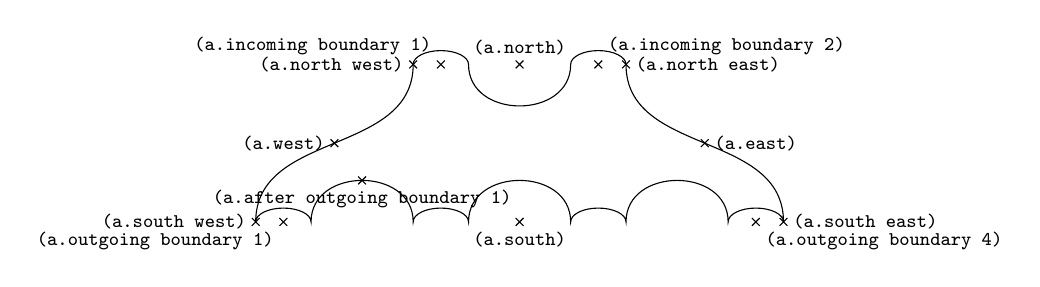
\begin{tikzpicture}
\node[tqft, incoming boundary components=2,outgoing boundary components=4,offset=-1,draw] (a) {};
\foreach \anchor/\placement in
{
north/above,
south/below,
east/right,
west/left,
north west/left,
south west/left,
north east/right,
south east/right,
incoming boundary 1/above left,
incoming boundary 2/above right,
outgoing boundary 1/below left,
outgoing boundary 4/below right,
after outgoing boundary 1/below}
\draw[shift=(a.\anchor)] plot[mark=x] coordinates{(0,0)} node[\placement] {\scriptsize\texttt{(a.\anchor)}};
\end{tikzpicture}
\end{example}

\begin{example}
\begin{tikzpicture}
\node[tqft,cylinder, circle width=2cm, circle depth=1cm, cobordism height=4cm,boundary separation=3cm,draw] (b) {};
\foreach \anchor/\placement in
{
prior/left,
next/right,
above/above,
below/below,
0/right,
60/right,
200/left}
\draw[shift=(b incoming 1.\anchor)] plot[mark=x] coordinates{(0,0)} node[\placement] {\scriptsize\texttt{(b incoming 1.\anchor)}};
\end{tikzpicture}
\end{example}

\section{Improvements}

Here are some ideas for extending this, and some minor ``bugs''.

\begin{enumerate}
\item Make \Verb+incoming boundary+ an alias of \Verb+incoming boundary 1+ so that if there is only one incoming boundary component then we don't need to specify the number (ditto outgoing).
\item No thought has been given as to where the text gets placed if it is specified.
\item Add the ability to hide certain boundary components.
This is useful if the shapes are not specified in their natural order so certain boundary components should be hidden behind earlier drawn shapes.
\item Some style options on the main node get passed to the other pieces (\Verb+fill opacity+ being one).
This shouldn't happen, or should happen by design not by accident.
\item The bounding box isn't as good as it could be.
\item Add a way to specify more directions for the flow.
\item Add the ability to apply different styles to the incoming and outgoing components.
\end{enumerate}

\section{More Examples}

\begin{example}
\begin{tikzpicture}[tqft/cobordism height=1.5cm,tqft/boundary  separation=1.5cm]
\foreach \coord/\style in {
{(0,0)}/{tqft/view from=outgoing,fill},
{(5,0)}/{tqft/view from=incoming,draw},
{(0,-8)}/{fill=orange,fill opacity=.5,tqft/boundary lower  style={draw,blue,ultra thin,dashed},tqft/boundary upper  style={draw,green},tqft/cobordism style={draw,purple},tqft/boundary  style={fill=yellow}},
{(5,-8)}/{fill=orange,fill opacity=.5,tqft/cobordism  style={draw,purple},tqft/boundary style={fill=yellow,draw=green}}
} {
\begin{scope}
\edef\styleit{\noexpand\tikzset{every node/.style={\style}}}
\styleit
\node[tqft/cap] (h) at \coord {};
\node[tqft/pair of pants,anchor=incoming boundary 1] (a) at  (h.outgoing boundary 1) {};
\node[tqft/cylinder to next,anchor=incoming boundary 1] (d) at  (a.incoming boundary 2) {};
\node[tqft/reverse pair of pants,anchor=incoming boundary 1] (b) at (a.outgoing boundary 2) {};
\node[tqft/cylinder to prior,anchor=incoming boundary 1] (c) at  (b.outgoing boundary 1) {};
\node[tqft/cylinder,anchor=incoming boundary 1] (e) at (a.outgoing  boundary 1) {};
\node[tqft/cylinder,anchor=incoming boundary 1] (f) at (e.outgoing  boundary 1) {};
\node[tqft/reverse pair of pants,anchor=incoming boundary 1] (g) at  (f.outgoing boundary 1) {};
\node[tqft/cup,anchor=incoming boundary 1] (i) at (g.outgoing boundary 1) {};
\end{scope}
}
\end{tikzpicture}
\end{example}

\begin{example}
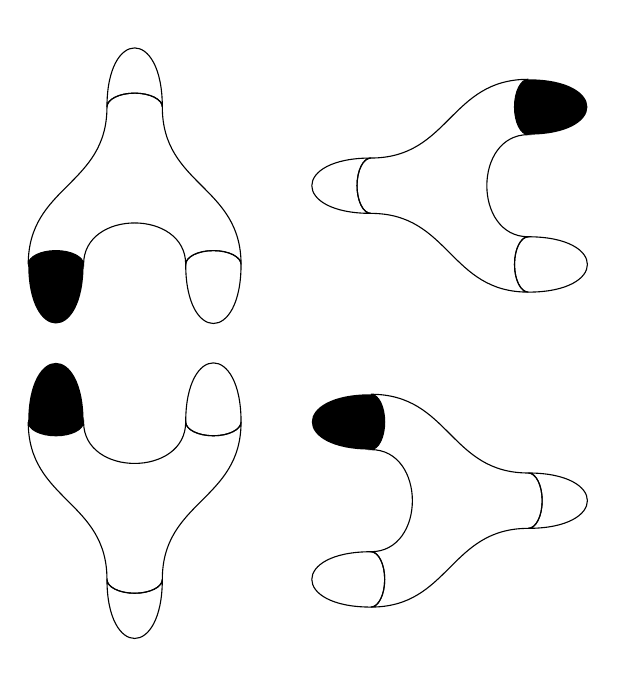
\begin{tikzpicture}
\node[draw,tqft/pair of pants] (a) {};
\node[draw,tqft/cap,anchor=outgoing boundary 1] at (a.incoming boundary 1) {};
\node[fill,tqft/cup,anchor=incoming boundary 1] at (a.outgoing boundary 1) {};
\node[draw,tqft/cup,anchor=incoming boundary 1] at (a.outgoing boundary 2) {};
\begin{scope}[tqft/flow=east]
\node[draw,tqft/pair of pants] (a) at (4,0) {};
\node[draw,tqft/cap,anchor=outgoing boundary 1] at (a.incoming boundary 1) {};
\node[fill,tqft/cup,anchor=incoming boundary 1] at (a.outgoing boundary 1) {};
\node[draw,tqft/cup,anchor=incoming boundary 1] at (a.outgoing boundary 2) {};
\end{scope}
\begin{scope}[tqft/flow=north]
\node[draw,tqft/pair of pants] (a) at (0,-4) {};
\node[draw,tqft/cap,anchor=outgoing boundary 1] at (a.incoming boundary 1) {};
\node[fill,tqft/cup,anchor=incoming boundary 1] at (a.outgoing boundary 1) {};
\node[draw,tqft/cup,anchor=incoming boundary 1] at (a.outgoing boundary 2) {};
\end{scope}
\begin{scope}[tqft/flow=west]
\node[draw,tqft/pair of pants] (a) at (4,-4) {};
\node[draw,tqft/cap,anchor=outgoing boundary 1] at (a.incoming boundary 1) {};
\node[fill,tqft/cup,anchor=incoming boundary 1] at (a.outgoing boundary 1) {};
\node[draw,tqft/cup,anchor=incoming boundary 1] at (a.outgoing boundary 2) {};
\end{scope}
\end{tikzpicture}
\end{example}

\end{document}